\documentclass[12pt,a4paper]{article}
\usepackage[top=2.5cm,bottom=2.5cm,left=2.5cm,right=2.5cm,headheight=15pt]{geometry}
\usepackage{amsmath,amssymb}
\usepackage{tikz}
\usetikzlibrary{shapes,arrows,arrows.meta,positioning,calc,backgrounds,fit,matrix}
\usepackage{booktabs,array,longtable,tabularx,multirow}
\usepackage{xcolor}
\usepackage{enumitem}
\usepackage{fancyhdr}
\usepackage{titlesec}
\usepackage{mdframed}
\usepackage{tcolorbox}
\tcbuselibrary{skins,breakable}
\usepackage{hyperref}

%% ---- Colors ----
\definecolor{folblue}{RGB}{0,82,165}
\definecolor{lightblue}{RGB}{220,235,255}
\definecolor{darkorange}{RGB}{180,70,0}
\definecolor{lightorange}{RGB}{255,235,210}
\definecolor{darkgreen}{RGB}{20,110,20}
\definecolor{lightgreen}{RGB}{200,240,205}
\definecolor{darkred}{RGB}{150,20,20}
\definecolor{lightred}{RGB}{255,210,210}
\definecolor{lightgray}{RGB}{242,242,242}

%% ---- tcolorbox styles ----
\newtcolorbox{qbox}[2][]{enhanced,breakable,
  colback=lightorange,colframe=darkorange,arc=4pt,
  title={\textbf{#2}},fonttitle=\bfseries\color{white},
  attach boxed title to top left={yshift=-2mm,xshift=4mm},
  boxed title style={colback=darkorange,arc=3pt},#1}

\newtcolorbox{solbox}[2][]{enhanced,breakable,
  colback=lightblue,colframe=folblue,arc=4pt,
  title={\textbf{#2}},fonttitle=\bfseries\color{white},
  attach boxed title to top left={yshift=-2mm,xshift=4mm},
  boxed title style={colback=folblue,arc=3pt},#1}

\newtcolorbox{keybox}[2][]{enhanced,breakable,
  colback=lightgreen,colframe=darkgreen,arc=4pt,
  title={\textbf{#2}},fonttitle=\bfseries\color{white},
  attach boxed title to top left={yshift=-2mm,xshift=4mm},
  boxed title style={colback=darkgreen,arc=3pt},#1}

\newtcolorbox{algobox}[2][]{enhanced,breakable,
  colback=lightgray,colframe=gray!60,arc=4pt,
  title={\textbf{#2}},fonttitle=\bfseries,
  attach boxed title to top left={yshift=-2mm,xshift=4mm},
  boxed title style={colback=gray!60,arc=3pt},#1}

\newtcolorbox{warnbox}[2][]{enhanced,breakable,
  colback=lightred,colframe=darkred,arc=4pt,
  title={\textbf{#2}},fonttitle=\bfseries\color{white},
  attach boxed title to top left={yshift=-2mm,xshift=4mm},
  boxed title style={colback=darkred,arc=3pt},#1}

%% ---- Page style ----
\pagestyle{fancy}\fancyhf{}
\lhead{\color{folblue}\textbf{Digital Signature --- CSE 717 InfoSec}}
\rhead{\color{folblue}Exam: 17 Jun 2026}
\cfoot{--- \thepage\ ---}
\renewcommand{\headrulewidth}{0.4pt}

%% ---- Section style ----
\titleformat{\section}{\large\bfseries\color{folblue}}{}{0em}{}[\titlerule]
\titleformat{\subsection}{\normalsize\bfseries\color{darkorange}}{}{0em}{}

\begin{document}

\begin{center}
{\LARGE\bfseries\color{folblue} CSE 717 --- Information Security}\\[4pt]
{\large\bfseries Topic 14: Digital Signature --- Generic Model, Properties, Vulnerabilities}\\[2pt]
{\large Complete Past Paper Solutions: 2020--2024}\\[6pt]
{\normalsize Source: general security knowledge (Stallings, Digital Signatures) --- partial Lc\#2 overlap (hash properties); diagram is a no-source cheat sheet}\\[2pt]
{\normalsize\color{darkred}\textbf{Every Topic-14 question 2020--2024 included. Zero omissions.}}
\end{center}

\tableofcontents
\newpage

%% ==========================================
\section*{Quick Reference --- The 5 Recurring Sub-Patterns (CHEAT SHEET)}
%% ==========================================

\begin{warnbox}{Diagram-heavy, low-prerequisite, CONFIRMED EVERY YEAR (5/5, 1--7 marks)}
Two recurring forms: (1) \textbf{draw the generic model} of the digital signature process (1--4.75 marks, pure diagram), and (2) \textbf{conceptual} questions on properties/attacks/requirements (3 marks). Combine with Topic 13 cheat sheet --- both are guaranteed, low-effort marks. ~30min investment.
\end{warnbox}

\begin{algobox}{1. What Is a Digital Signature?}
A \textbf{digital signature} is a cryptographic value, computed from a message and the sender's \textbf{private key}, that is attached to the message to provide:
\begin{itemize}[noitemsep]
  \item \textbf{Authentication} --- proves the message came from the claimed sender.
  \item \textbf{Integrity} --- proves the message was not altered in transit.
  \item \textbf{Non-repudiation} --- the sender cannot later deny having sent the message.
\end{itemize}
\textbf{Key idea:} the signer's private key is used to ``sign'' (encrypt a hash of the message), and anyone holding the corresponding \textbf{public key} can verify the signature --- but only the signer could have produced it.
\end{algobox}

\begin{algobox}{2. Generic Model of the Digital Signature Process}
\textbf{Sender side:}
\begin{enumerate}[noitemsep]
  \item Compute a hash of the message: $h = H(M)$.
  \item Encrypt the hash with the sender's \textbf{private key} $PR_a$: $DS = E_{PR_a}(h)$. This $DS$ is the digital signature.
  \item Send $(M, DS)$ to the receiver.
\end{enumerate}
\textbf{Receiver side:}
\begin{enumerate}[noitemsep]
  \item Decrypt $DS$ using the sender's \textbf{public key} $PU_a$ to recover $h$: $h = D_{PU_a}(DS)$.
  \item Independently compute $h' = H(M)$ on the received message.
  \item \textbf{Compare} $h \stackrel{?}{=} h'$: if equal $\to$ signature valid (message authentic \& unmodified); if not $\to$ reject.
\end{enumerate}

\begin{center}
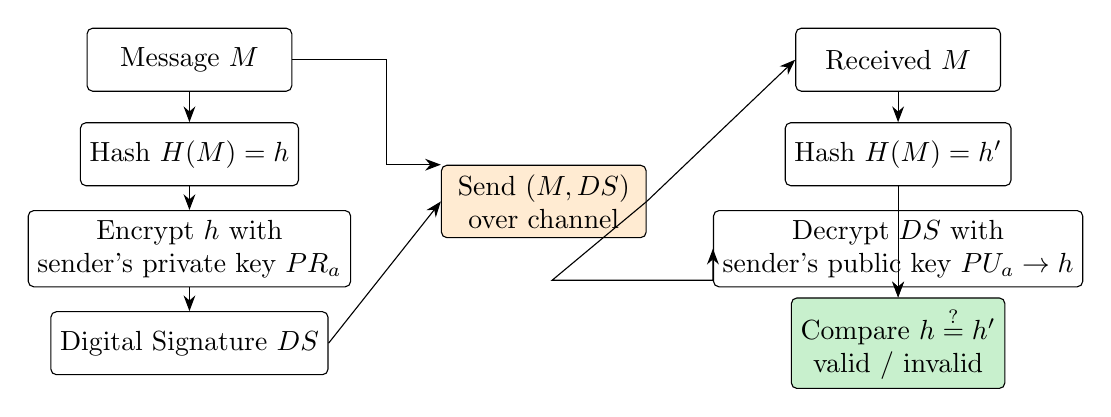
\begin{tikzpicture}[
  box/.style={draw, rectangle, minimum width=2.6cm, minimum height=0.8cm, align=center, rounded corners=2pt},
  >={Stealth[length=2mm]}, node distance=0.9cm
]
  % Sender column
  \node[box] (M1) at (0,4) {Message $M$};
  \node[box] (H1) at (0,2.8) {Hash $H(M)=h$};
  \node[box] (E1) at (0,1.6) {Encrypt $h$ with\\sender's private key $PR_a$};
  \node[box] (DS) at (0,0.4) {Digital Signature $DS$};

  % Channel
  \node[box,fill=lightorange] (CH) at (4.5,2.2) {Send $(M, DS)$\\over channel};

  % Receiver column
  \node[box] (M2) at (9,4) {Received $M$};
  \node[box] (H2) at (9,2.8) {Hash $H(M)=h'$};
  \node[box] (D2) at (9,1.6) {Decrypt $DS$ with\\sender's public key $PU_a \to h$};
  \node[box,fill=lightgreen] (CMP) at (9,0.4) {Compare $h \stackrel{?}{=} h'$\\valid / invalid};

  \draw[->] (M1) -- (H1);
  \draw[->] (H1) -- (E1);
  \draw[->] (E1) -- (DS);
  \draw[->] (DS.east) -- (CH.west);
  \draw[->] (M1.east) -- ++(1.2,0) |- (CH.north west);
  \draw[->] (CH.east) -- (M2.west);
  \draw[->] (CH.east) -- ++(-1.2,-1.0) -| (D2.west);
  \draw[->] (M2) -- (H2);
  \draw[->] (D2) -- (CMP);
  \draw[->] (H2) -- (CMP);
\end{tikzpicture}
\end{center}
\end{algobox}

\begin{algobox}{3. Properties / Requirements of a Digital Signature Scheme}
\textbf{A digital signature must:}
\begin{itemize}[noitemsep]
  \item \textbf{Verify the author} and the date/time of the signature.
  \item \textbf{Authenticate the contents} at the time of signing.
  \item Be \textbf{verifiable by third parties}, to resolve disputes.
\end{itemize}
\textbf{Practical requirements on the signature itself:}
\begin{itemize}[noitemsep]
  \item Must be a bit pattern that \textbf{depends on the message} being signed.
  \item Must use information \textbf{unique to the sender} (the private key) --- to prevent both forgery and denial.
  \item Must be \textbf{relatively easy to produce}.
  \item Must be \textbf{relatively easy to recognize and verify}.
  \item Must be \textbf{computationally infeasible to forge} --- either (a) by constructing a new message for an existing signature, or (b) by constructing a fraudulent signature for a given message.
  \item Must be \textbf{practical to retain a copy} of the digital signature in storage.
\end{itemize}
\end{algobox}

\begin{algobox}{4. Attack / Forgery Types Vulnerable to Digital Signatures}
\begin{itemize}[noitemsep]
  \item \textbf{Key-only attack:} attacker only knows the signer's public key.
  \item \textbf{Known-message attack:} attacker has a set of previously signed messages.
  \item \textbf{Chosen-message attack:} attacker can choose messages and obtain valid signatures for them (generic / directed / adaptive variants).
\end{itemize}
\textbf{Resulting forgery outcomes:}
\begin{itemize}[noitemsep]
  \item \textbf{Total break:} attacker recovers the signer's private key.
  \item \textbf{Universal forgery:} attacker can forge a signature for \emph{any} message.
  \item \textbf{Selective forgery:} attacker can forge a signature for \emph{one chosen} message.
  \item \textbf{Existential forgery:} attacker can produce \emph{at least one} valid (message, signature) pair not previously seen --- weakest but still a break of security.
\end{itemize}
\end{algobox}

\begin{algobox}{5. Direct Digital Signature: Order vs. Confidentiality + Threats}
\textbf{Order of signature vs.\ confidentiality function:}
\begin{itemize}[noitemsep]
  \item \textbf{Sign-then-encrypt} (preferred): sign the plaintext message first, then encrypt \emph{both} the message and its signature with a shared secret key. The signature is now protected inside the encrypted envelope, and disputes can later be resolved using the original (unencrypted) signed message.
  \item \textbf{Encrypt-then-sign} is generally discouraged: a third party verifying the signature would need access to the plaintext, weakening confidentiality.
\end{itemize}
\textbf{Threats to a \emph{direct} digital signature scheme} (security depends entirely on the sender's private key):
\begin{enumerate}[noitemsep]
  \item \textbf{Key compromise (forgery):} if the sender's private key is actually stolen, the attacker can forge the sender's signature on new messages.
  \item \textbf{Repudiation via false claim:} the sender can falsely claim their private key was lost/stolen at some earlier time, to disown a signature they actually created (denial of responsibility).
\end{enumerate}
\textbf{Mitigation:} timestamps + a trusted third party (e.g.\ arbitration/notarization) to bind signatures to a verified time.
\end{algobox}

\begin{algobox}{Bonus: RSA --- Safety After a Private-Key Leak (2023 Section B Q5(d))}
If a user's RSA \textbf{private key is leaked}:
\begin{itemize}[noitemsep]
  \item \textbf{Past encrypted messages are NOT safe} --- an attacker who recorded old ciphertexts can now decrypt all of them with the leaked private key (RSA, as used here, provides \textbf{no forward secrecy}).
  \item \textbf{Past signatures become untrustworthy} --- the attacker could forge new signatures claiming to be from a past date, and the legitimate signer can plausibly deny old signatures (repudiation risk).
  \item \textbf{Conclusion:} reusing the same RSA key pair indefinitely is \textbf{not safe} once compromised --- keys must be revoked/rotated immediately, and a certificate revocation mechanism (CRL/OCSP) is needed.
\end{itemize}
\end{algobox}

\newpage
%% ==========================================
\section{2024 --- Q2(a): Digital Signature + Vulnerable Attacks (3); Section B Q2(c): Same Theme (3); Section B Q8(d): Generic Model Diagram (1)}
%% ==========================================

\begin{qbox}{Question --- 2024 Q2(a) and Section B Q2(c)}
What is a digital signature? What types of attacks make digital signatures vulnerable? \hfill [3 + 3]
\end{qbox}

\begin{solbox}{Answer --- 2024 Q2(a) / Section B Q2(c)}
\textbf{What is a digital signature:} see Cheat Sheet \#1 --- a value computed from the message and the sender's private key, attached to provide \textbf{authentication}, \textbf{integrity}, and \textbf{non-repudiation}.

\textbf{Attack types that make it vulnerable:} see Cheat Sheet \#4:
\begin{itemize}[noitemsep]
  \item \textbf{Key-only}, \textbf{known-message}, and \textbf{chosen-message} attacks (generic/directed/adaptive).
  \item Resulting forgeries: \textbf{total break}, \textbf{universal}, \textbf{selective}, \textbf{existential forgery}.
\end{itemize}
\end{solbox}

\begin{qbox}{Question --- 2024 Section B Q8(d)}
Draw the generic model of the digital signature process. \hfill [1]
\end{qbox}

\begin{solbox}{Answer --- 2024 Section B Q8(d)}
See Cheat Sheet \#2 diagram: \textbf{sender} hashes $M \to h$, encrypts $h$ with private key $PR_a$ to get $DS$, sends $(M,DS)$; \textbf{receiver} decrypts $DS$ with public key $PU_a$ to recover $h$, independently hashes received $M$ to get $h'$, and \textbf{compares} $h$ vs $h'$.
\end{solbox}

\newpage
%% ==========================================
\section{2023 --- Q2(a): Digital Signature + Vulnerable Attacks (3); Section B Q5(c): Attack Types (3); Section B Q5(d): RSA Key-Reuse Safety (1)}
%% ==========================================

\begin{qbox}{Question --- 2023 Q2(a) and Section B Q5(c,d)}
\begin{enumerate}[label=(\alph*)]
  \item What is a digital signature? What types of attacks make it vulnerable? \hfill [3]
  \item (Section B Q5(c)) What attack types is a digital signature vulnerable to? \hfill [3]
  \item (Section B Q5(d)) If a user's RSA private key is leaked, is reusing the same key pair safe? \hfill [1]
\end{enumerate}
\end{qbox}

\subsection{Parts (a) and Section B (c): Digital Signature + Attacks}
\begin{solbox}{Answer --- 2023 Q2(a) / Section B Q5(c)}
Identical content to 2024 Q2(a) above --- see Cheat Sheet \#1 (definition: authentication, integrity, non-repudiation) and Cheat Sheet \#4 (key-only / known-message / chosen-message attacks $\to$ total break / universal / selective / existential forgery).
\end{solbox}

\subsection{Part Section B (d): RSA Key-Reuse Safety After Private-Key Leak}
\begin{solbox}{Answer --- 2023 Section B Q5(d)}
See Cheat Sheet (Bonus): \textbf{NO} --- a leaked RSA private key means:
\begin{itemize}[noitemsep]
  \item All \textbf{past ciphertexts} (recorded by an eavesdropper) can now be decrypted --- \textbf{no forward secrecy}.
  \item All \textbf{past signatures} become questionable --- attacker can forge new ones, legitimate owner can deny old ones.
  \item The key pair must be \textbf{revoked and rotated immediately}; continuing to use it is unsafe.
\end{itemize}
\end{solbox}

\newpage
%% ==========================================
\section{2022 --- Section B Q5(b): Properties + Scheme Requirements; Q7(a): Signature vs Confidentiality Order + Threats to Direct DS}
%% ==========================================

\begin{qbox}{Question --- 2022 Section B Q5(b) and Q7(a)}
\begin{enumerate}[label=(\alph*)]
  \item (Section B Q5(b)) What properties should a digital signature have? What are the requirements for a digital signature scheme?
  \item (Q7(a)) What is the correct order of applying the signature function and the confidentiality function? What are the threats to a direct digital signature scheme?
\end{enumerate}
\end{qbox}

\subsection{Part (a): Properties + Scheme Requirements}
\begin{solbox}{Answer --- 2022 Section B Q5(b)}
See Cheat Sheet \#3 in full:
\begin{itemize}[noitemsep]
  \item \textbf{Properties:} must verify author + date/time, authenticate contents at signing time, be verifiable by third parties to resolve disputes.
  \item \textbf{Scheme requirements:} signature depends on the message; uses sender-unique info (private key); easy to produce \& verify; computationally infeasible to forge; practical to store.
\end{itemize}
\end{solbox}

\subsection{Part (b): Signature vs Confidentiality Order + Threats to Direct Digital Signature}
\begin{solbox}{Answer --- 2022 Q7(a)}
See Cheat Sheet \#5:
\begin{itemize}[noitemsep]
  \item \textbf{Correct order:} \textbf{sign-then-encrypt} --- sign the plaintext message, then encrypt the message+signature together with a shared secret key. (Encrypt-then-sign weakens confidentiality, since verifiers would need plaintext access.)
  \item \textbf{Threats to direct digital signature} (security rests entirely on the sender's private key):
  \begin{enumerate}[noitemsep]
    \item \textbf{Key compromise} --- stolen private key lets an attacker forge the sender's signature.
    \item \textbf{False repudiation} --- sender falsely claims the key was stolen earlier, to disown a genuine signature.
  \end{enumerate}
  \textbf{Mitigation:} timestamps + a trusted third party (arbitration).
\end{itemize}
\end{solbox}

\newpage
%% ==========================================
\section{2021 --- Section B Q2(c): Generic Model Diagram (2 marks)}
%% ==========================================

\begin{qbox}{Question --- 2021 Section B Q2(c)}
Draw the generic model of the digital signature process. \hfill [2]
\end{qbox}

\begin{solbox}{Answer --- 2021 Section B Q2(c)}
Same diagram as Cheat Sheet \#2: \textbf{sender} $M \xrightarrow{H} h \xrightarrow{\text{encrypt with } PR_a} DS$, send $(M,DS)$; \textbf{receiver} decrypts $DS$ with $PU_a \to h$, hashes received $M \to h'$, \textbf{compares} $h$ vs $h'$ to validate.
\end{solbox}

\newpage
%% ==========================================
\section{2020 --- Q7(a): Generic Model of Digital Signature Process (4.75 marks)}
%% ==========================================

\begin{qbox}{Question --- 2020 Q7(a)}
Draw and explain the generic model of the digital signature process. \hfill [4.75]
\end{qbox}

\begin{solbox}{Answer --- 2020 Q7(a)}
Same diagram + explanation as Cheat Sheet \#2 --- this is the highest-mark version (4.75), so write out \textbf{all 6 steps} explicitly (3 sender-side + 3 receiver-side):
\begin{enumerate}[noitemsep]
  \item Sender computes $h = H(M)$.
  \item Sender encrypts $h$ with private key $PR_a$ to get $DS$.
  \item Sender transmits $(M, DS)$.
  \item Receiver decrypts $DS$ with sender's public key $PU_a$ to recover $h$.
  \item Receiver independently computes $h' = H(M)$ on the received message.
  \item Receiver compares $h$ vs $h'$ --- equal $\Rightarrow$ authentic \& unmodified; not equal $\Rightarrow$ reject.
\end{enumerate}
Plus the diagram from Cheat Sheet \#2.
\end{solbox}

\newpage
%% ==========================================
\section*{Exam Strategy Summary}
%% ==========================================

\begin{keybox}{High-Yield Checklist for Digital Signature (5/5 years, 1--7 marks --- GUARANTEED)}
\begin{enumerate}[noitemsep]
  \item \textbf{Generic model diagram} (sender hashes $\to$ encrypt with private key $\to$ DS; receiver decrypts with public key, re-hashes, compares) --- asked EVERY year (2020, 2021, 2024) in some form. Practice drawing it from memory in under 2 minutes.
  \item \textbf{Definition + vulnerable attack types} (key-only / known-message / chosen-message $\to$ total break / universal / selective / existential forgery) --- asked 2023, 2024.
  \item \textbf{Properties + scheme requirements} (verify author/date, authenticate contents, third-party verifiable; signature depends on message, uses private key, easy to produce/verify, infeasible to forge, practical to store) --- asked 2022.
  \item \textbf{Sign-then-encrypt order + threats to direct DS} (key compromise, false repudiation; mitigated by timestamps + trusted third party) --- asked 2022.
  \item \textbf{RSA private-key leak $\Rightarrow$ no forward secrecy, revoke \& rotate} --- asked 2023, cheap 1 mark.
\end{enumerate}
\textit{Total: ~30 minutes of focused memorization for 1--7 GUARANTEED marks every single year. Pairs naturally with Topic 13 (DES/Feistel) cheat sheet.}
\end{keybox}

\end{document}
